\let\negmedspace\undefined
\let\negthickspace\undefined
\documentclass[journal,12pt,onecolumn]{IEEEtran}
\usepackage{cite}
\usepackage{amsmath,amssymb,amsfonts,amsthm}
\usepackage{algorithmic}
\usepackage{graphicx}
\usepackage{textcomp}
\usepackage{xcolor}
\usepackage{txfonts}
\usepackage{listings}
\usepackage{enumitem}
\usepackage{mathtools}
\usepackage{gensymb}
\usepackage{comment}
\usepackage[breaklinks=true]{hyperref}
\usepackage{tkz-euclide} 
\usepackage{gvv}                                        
                              
\usepackage[latin1]{inputenc}     
\usepackage{xparse}
\usepackage{color}                                            
\usepackage{array}                                            
\usepackage{longtable}                                       
\usepackage{calc}                                             
\usepackage{multirow}
\usepackage{multicol}
\usepackage{hhline}                                           
\usepackage{ifthen}                                           
\usepackage{lscape}
\usepackage{tabularx}
\usepackage{float}
\newtheorem{theorem}{Theorem}[section]
\newtheorem{problem}{Problem}
\newtheorem{proposition}{Proposition}[section]
\newtheorem{lemma}{Lemma}[section]
\newtheorem{corollary}[theorem]{Corollary}
\newtheorem{example}{Example}[section]
\newtheorem{definition}[problem]{Definition}
\newcommand{\BEQA}{\begin{eqnarray}}
\newcommand{\EEQA}{\end{eqnarray}}
\newcommand{\define}{\stackrel{\triangle}{=}}
\theoremstyle{remark}
\newtheorem{rem}{Remark}

\begin{document}
\title{PI :CIVIL ENGINEERING}
\author{AI25BTECH11034 - Sujal Chauhan}
\maketitle
\renewcommand{\thefigure}{\theenumi}
\renewcommand{\thetable}{\theenumi}

    
\begin{center}
    

\vspace{6cm}
\textbf{\LARGE SESSION 1}
\end{center}
\newpage
\textbf{\large Q.1 - Q.5 carry one mark each}
\begin{enumerate}
% Q.1
\item The driver applied the \underline{\hspace{2cm}} as soon as she approached the hotel where she wanted to take a \underline{\hspace{2cm}}.''
\\The words that best fill the blanks in the above sentence are\hfill{(GATE 2018)}
\begin{multicols}{4}
\begin{enumerate}
    \item brake, break
    \item break, break
    \item brake, brake
    \item break, brake
\end{enumerate}
\end{multicols}
\vspace{1cm}

% Q.2
\item ``It is no surprise that every society has had codes of behaviour; however, the nature of these codes is often \underline{\hspace{2cm}}.''\hfill{(GATE 2018)}
\\The word that best fills the blank in the above sentence is
\begin{multicols}{4}
\begin{enumerate}
    \item unpredictable
    \item simple
    \item expected
    \item strict
\end{enumerate}
\end{multicols}
\vspace{1cm}

% Q.3
\item Hemaa's age is 5 years more than twice Hari's age. Suresh's age is 13 years less than 10 times Hari's age. If Suresh is 3 times as old as Hema, how old is Hema?\hfill{(GATE 2018)}
\begin{multicols}{4}
\begin{enumerate}
    \item 14
    \item 17
    \item 18
    \item 19
\end{enumerate}
\end{multicols}
\vspace{1cm}

% Q.4
\item Tower A is 90 m tall and tower B is 140 m tall. They are 100 m apart. A horizontal skywalk connects the floors at 70 m in both the towers. If a taut rope connects the top of tower A to the bottom of tower B, at what distance (in meters) from tower A will the rope intersect the skywalk?\hfill{(GATE 2018)}
\begin{multicols}{4}
\begin{enumerate}
    \item 22.22
    \item 50
    \item 57.87
    \item 77.78
\end{enumerate}
\end{multicols}
\vspace{1cm}

% Q.5
\item The temperature $T$ in a room varies as a function of the outside temperature $T_0$ and the number of persons in the room $p$, according to the relation $T = K (\Theta p + T_0)$, where $\Theta$ and $K$ are constants. What would be the value of $\Theta$ given the following data?\hfill{(GATE 2018)}
\\
\[
\begin{array}{|c|c|c|}
\hline
T_0 & p & T \\
\hline
25 & 2 & 32.4 \\
30 & 5 & 42.0 \\
\hline
\end{array}
\]
\begin{multicols}{4}
\begin{enumerate}
    \item 0.8
    \item 1.0
    \item 2.0
    \item 10.0
\end{enumerate}
\end{multicols}
\vspace{1cm}
\newpage
\textbf{\large Q.6 - Q.10 carry two mark each}
% Q.6
\item A fruit seller sold a basket of fruits at 12.5\% loss. Had he sold it for Rs. 108 more, he would have made a 10\% gain. What is the loss in Rupees incurred by the fruit seller?\hfill{(GATE 2018)}
\begin{multicols}{4}
\begin{enumerate}
    \item 48
    \item 52
    \item 60
    \item 108
\end{enumerate}
\end{multicols}
\vspace{1cm}

% Q.7
\item The price of a wire made of a superalloy material is proportional to the square of its length. The price of 10 m length of the wire is Rs. 1600. What would be the total price (in Rs.) of two wires of lengths 4 m and 6 m?\hfill{(GATE 2018)}
\begin{multicols}{4}
\begin{enumerate}
    \item 768
    \item 832
    \item 1440
    \item 1600
\end{enumerate}
\end{multicols}
\vspace{1cm}

% Q.8
\item Which of the following function(s) is an accurate description of the graph for the range(s) indicated?
\hfill{(GATE 2018)}
\begin{figure}[h]
    \centering
    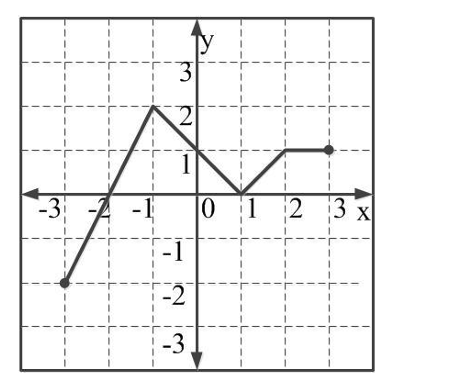
\includegraphics[width=0.5\linewidth]{GATE-CE-2018/8A-1.png}
    \caption{}
    \label{8a-1}
\end{figure}
(i) $y = 2x + 4$ for $-3 \leq x \leq -1$ \\
(ii) $y = |x-1|$ for $-1 \leq x \leq 2$ \\
(iii) $y = ||x|-1|$ for $-1 \leq x \leq 2$ \\
(iv) $y = 1$ for $2 \leq x \leq 3$ 
\begin{multicols}{4}
\begin{enumerate}
    \item (i), (ii) and (iii) only.
    \item (i), (ii) and (iv) only.
    \item (i) and (iv) only.
    \item (ii) and (iv) only.
\end{enumerate}
\end{multicols}
\vspace{1cm}
\newpage
% Q.9
\item Consider a sequence of numbers $a_1, a_2, a_3, \ldots, a_n$ where $a_n = \frac{1}{n} - \frac{1}{n+2}$ for each integer $n > 0$. What is the sum of the first 50 terms?\hfill{(GATE 2018)}
\begin{multicols}{4}
\begin{enumerate}
    \item $\left(1 + \frac{1}{2}\right) - \frac{1}{50}$
    \item $\left(1 + \frac{1}{2}\right) + \frac{1}{50}$
    \item $\left(1 + \frac{1}{2}\right) - \left(\frac{1}{51} + \frac{1}{52}\right)$
    \item $1 - \left(\frac{1}{51} + \frac{1}{52}\right)$
\end{enumerate}
\end{multicols}
\vspace{1cm}

% Q.10
\item Each of the letters arranged as below represents a unique integer from 1 to 9. The letters are positioned in the figure such that $(A \times B \times C)$, $(B \times G \times E)$ and $(D \times E \times F)$ are equal. Which integer among the following choices cannot be represented by the letters A, B, C, D, E, F or G?\hfill{(GATE 2018)}
\[
\begin{array}{ccc}
A &   & D \\
B & G & E \\
C &   & F \\
\end{array}
\]
\begin{multicols}{4}
\begin{enumerate}
    \item 4
    \item 5
    \item 6
    \item 9
\end{enumerate}
\end{multicols}
\vspace{1cm}









\end{enumerate}

\newpage
\textbf{\large Q.1 - Q.25 carry one mark each}
\begin{enumerate}
  \vspace{1cm}
  % Q.1
\item Which one of the following matrices is singular?
\hfill{(GATE 2018)}
\begin{multicols}{4}
\begin{enumerate}
    \item $\myvec{ 2 & 5 \\ 1 & 3 }$
    \item $\myvec{ 3 & 2 \\ 2 & 3 }$
    \item $\myvec{ 2 & 4 \\ 3 & 6 }$
    \item $\myvec{ 4 & 3 \\ 6 & 2 }$
\end{enumerate}
\end{multicols}
\vspace{1cm}

% Q.2
\item For the given orthogonal matrix $Q$,
\[
Q =
\myvec{
3/7 & 2/7 & 6/7 \\
-6/7 & 3/7 & 2/7 \\
2/7 & 6/7 & -3/7
}
\]
The inverse is\hfill{(GATE 2018)}
\begin{multicols}{4}
\begin{enumerate}
    \item
    $\myvec{
    3/7 & 2/7 & 6/7 \\
    -6/7 & 3/7 & 2/7 \\
    2/7 & 6/7 & -3/7
    }$
    \item
    $\myvec{
    -3/7 & -2/7 & -6/7 \\
    6/7 & -3/7 & -2/7 \\
    -2/7 & -6/7 & 3/7
    }$
    \item
    $\myvec{
    3/7 & -6/7 & 2/7 \\
    2/7 & 3/7 & 6/7 \\
    6/7 & 2/7 & -3/7
    }$
    \item
    $\myvec{
    -3/7 & 6/7 & -2/7 \\
    2/7 & -3/7 & -6/7 \\
    -6/7 & -2/7 & 3/7
    }$
\end{enumerate}
\end{multicols}
\vspace{1cm}

% Q.3
\item At the point $x=0$, the function $f(x)=x^3$ has\hfill{(GATE 2018)}
\begin{multicols}{4}
\begin{enumerate}
    \item local maximum
    \item local minimum
    \item both local maximum and minimum
    \item neither local maximum nor local minimum
\end{enumerate}
\end{multicols}
\vspace{1cm}

% Q.4
\item A column of height $h$ with a rectangular cross-section of size $a \times 2a$ has a buckling load of $P$. If the cross-section is changed to $0.5a \times 3a$ and its height changed to $1.5h$, the buckling load of the redesigned column will be\hfill{(GATE 2018)}
\begin{multicols}{4}
\begin{enumerate}
    \item $P/12$
    \item $P/4$
    \item $P/2$
    \item $3P/4$
\end{enumerate}
\end{multicols}
\vspace{1cm}
% Q.5
\item A steel column of ISHB 350 @72.4 kg/m is subjected to a factored axial compressive load of 2000 kN. The load is transferred to a concrete pedestal of grade M20 through a square base plate. Consider bearing strength of concrete as $0.45 f_{ck}$, where $f_{ck}$ is the characteristic strength of concrete. Using limit state method and neglecting the self weight of base plate and steel column, the length of a side of the base plate to be provided is\hfill{(GATE 2018)}
\begin{multicols}{4}
\begin{enumerate}
    \item 39 cm
    \item 42 cm
    \item 45 cm
    \item 48 cm
\end{enumerate}
\end{multicols}
\vspace{1cm}
\newpage

% Q.6
\item The Le Chatelier apparatus is used to determine\hfill{(GATE 2018)}
\begin{multicols}{4}
\begin{enumerate}
    \item compressive strength of cement
    \item fineness of cement
    \item setting time of cement
    \item soundness of cement
\end{enumerate}
\end{multicols}
\vspace{1cm}

% Q.7
\item The deformation in concrete due to sustained loading is\hfill{(GATE 2018)}
\begin{multicols}{4}
\begin{enumerate}
    \item creep
    \item hydration
    \item segregation
    \item shrinkage
\end{enumerate}
\end{multicols}
\vspace{1cm}

% Q.8
\item A solid circular beam with radius of 0.25~m and length of 2~m is subjected to a twisting moment of 20~kNm about the z-axis at the free end, which is the only load acting as shown in the figure. The shear stress component $\tau_{xy}$ at Point `M' in the cross-section of the beam at a distance of 1~m from the fixed end is\hfill{(GATE 2018)}
\begin{multicols}{4}
\begin{enumerate}
    \item 0.0 MPa
    \item 0.51 MPa
    \item 0.815 MPa
    \item 2.0 MPa
\end{enumerate}
\end{multicols}
\vspace{1cm}

% Q.9
\item Two rectangular under-reinforced concrete beam sections X and Y are similar in all aspects except that the longitudinal compression reinforcement in section Y is 10\% more. Which one of the following is the correct statement?\hfill{(GATE 2018)}
\begin{multicols}{4}
\begin{enumerate}
    \item Section X has less flexural strength and is less ductile than section Y
    \item Section X has less flexural strength but is more ductile than section Y
    \item Sections X and Y have equal flexural strength but different ductility
    \item Sections X and Y have equal flexural strength and ductility
\end{enumerate}
\end{multicols}
\vspace{1cm}

% Q.10
\item The percent reduction in the bearing capacity of a strip footing resting on sand under flooding condition (water level at the base of the footing) when compared to the situation where the water level is at a depth much greater than the width of footing, is approximately\hfill{(GATE 2018)}
\begin{multicols}{4}
\begin{enumerate}
    \item 0
    \item 25
    \item 50
    \item 100
\end{enumerate}
\end{multicols}
\vspace{1cm}

% Q.11
\item The width of a square footing and the diameter of a circular footing are equal. If both the footings are placed on the surface of sandy soil, the ratio of the ultimate bearing capacity of circular footing to that of square footing will be\hfill{(GATE 2018)}
\begin{multicols}{4}
\begin{enumerate}
    \item 4/3
    \item 1
    \item 3/4
    \item 2/3
\end{enumerate}
\end{multicols}
\vspace{1cm}
\newpage
% Q.12
\item Bernoulli's equation is applicable for\hfill{(GATE 2018)}

\begin{enumerate}
    \item viscous and compressible fluid flow
    \item inviscid and compressible fluid flow
    \item inviscid and incompressible fluid flow
    \item viscous and incompressible fluid flow
\end{enumerate}

\vspace{1cm}

% Q.13
\item There are 20,000 vehicles operating in a city with an average annual travel of 12,000 km per vehicle. The NOx emission rate is 2.0 g/km per vehicle. The total annual release of NOx will be\hfill{(GATE 2018)}
\begin{multicols}{4}
\begin{enumerate}
    \item 4,80,000 kg
    \item 4,800 kg
    \item 480 kg
    \item 48 kg
\end{enumerate}
\end{multicols}
\vspace{1cm}

% Q.14
\item A bitumen sample has been graded as VG30 as per IS : 73-2013. The 30 in the grade means that \hfill{(GATE 2018)}

\begin{enumerate}
    \item penetration of bitumen at $25^\circ$C is between 20 and 40
    \item viscosity of bitumen at $60^\circ$C is between 2400 and 3600 Poise
    \item ductility of bitumen at $27^\circ$C is more than 30 cm
    \item elastic recovery of bitumen at $15^\circ$C is more than 30\%
\end{enumerate}

\vspace{1cm}

% Q.15
\item The speed-density relationship for a road section is shown in the figure. \hfill{(GATE 2018)}
\begin{figure}[h]
    \centering
    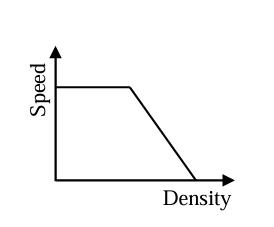
\includegraphics[width=0.5\linewidth]{GATE-CE-2018/15-1.png}
    \caption{}
    \label{15-1}
\end{figure}
The shape of the flow-density relationship is

\begin{enumerate}
    \item piecewise linear
    \item parabolic
    \item initially linear then parabolic
    \item initially parabolic then linear
\end{enumerate}

\vspace{1cm}
\newpage
% Q.16
\item A well-designed signalized intersection is one in which the \hfill{(GATE 2018)}

\begin{enumerate}
    \item crossing conflicts are increased
    \item total delay is minimized
    \item cycle time is equal to the sum of red and green times in all phases
    \item cycle time is equal to the sum of red and yellow times in all phases
\end{enumerate}

\vspace{1cm}
% Q.17
\item A flow field is given by $u = y^2$, $v = -xy$, $w = 0$. Value of the $z$-component of the angular velocity (in radians per unit time, up to two decimal places) at the point $(0,-1,1)$ is \underline{\hspace{3cm}} 
\hfill{(GATE 2018)}
\vspace{1cm}

% Q.18
\item The frequency distribution of the compressive strength of 20 concrete cube specimens is given in the table.
\[
\begin{array}{|c|c|}
\hline
f\,(\text{MPa}) & \text{Number of specimens with compressive strength equal to}\, f \\
\hline
23 & 4 \\
28 & 2 \\
22.5 & 5 \\
31 & 5 \\
29 & 4 \\
\hline
\end{array}
\]
If $\mu$ is the mean strength of the specimens and $\sigma$ is the standard deviation, the number of specimens (out of 20) with compressive strength less than $\mu - 3\sigma$ is \underline{\hspace{3cm}}
\hfill{(GATE 2018)}
\vspace{1cm}

% Q.19
\item In a fillet weld, the direct shear stress and bending tensile stress are $50$ MPa and $150$ MPa, respectively. As per IS 800: 2007, the equivalent stress (in MPa, up to two decimal places) will be \underline{\hspace{3cm}}
\hfill{(GATE 2018)}
\vspace{1cm}

% Q.20
\item In a shrinkage limit test, the volume and mass of a dry soil pat are found to be $50$ cm$^3$ and $88$ g, respectively. The specific gravity of the soil solids is $2.71$ and the density of water is $1$ g/cc. The shrinkage limit (in \%, up to two decimal places) is \underline{\hspace{3cm}}
\hfill{(GATE 2018)}
\vspace{1cm}

% Q.21
\item A core cutter of $130$ mm height has inner and outer diameters of $100$ mm and $106$ mm, respectively. The area ratio of the core cutter (in \%, up to two decimal places) is \underline{\hspace{3cm}}
\hfill{(GATE 2018)}
\vspace{1cm}

% Q.22
\item A 1:50 model of a spillway is to be tested in the laboratory. The discharge in the prototype spillway is $1000$ m$^3$/s. The corresponding discharge (in m$^3$/s, up to two decimal places) to be maintained in the model, neglecting variation in acceleration due to gravity, is \underline{\hspace{3cm}}
\hfill{(GATE 2018)}
\vspace{1cm}

% Q.23
\item A $10$ m wide rectangular channel carries a discharge of $20$ m$^3$/s under critical condition. Using $g = 9.81$ m/s$^2$, the specific energy (in m, up to two decimal places) is \underline{\hspace{3cm}}
\hfill{(GATE 2018)}
\vspace{1cm}

% Q.24
\item For routing of flood in a given channel using the Muskingum method, two of the routing coefficients are estimated as $C_0 = -0.25$ and $C_1 = 0.55$. The value of the third coefficient $C_2$ would be \underline{\hspace{3cm}}
\hfill{(GATE 2018)}
\vspace{1cm}

% Q.25
\item A city generates $40 \times 10^6$ kg of municipal solid waste (MSW) per year, out of which only 10\% is recovered/recycled and the rest goes to landfill. The landfill has a single lift of $3$ m height and is compacted to a density of $550$ kg/m$^3$. If 80\% of the landfill is assumed to be MSW, the landfill area (in m$^2$, up to one decimal place) required would be \underline{\hspace{3cm}}
\hfill{(GATE 2018)}
\vspace{1cm}
\newpage
\textbf{\large Q.26 - Q.55 carry two mark each}
\vspace{1cm}
% Q.26
\item The value of the integral $\int_{0}^{\pi} x \cos^2 x dx$ is
\hfill{(GATE 2018)}
\begin{multicols}{4}
\begin{enumerate}
    \item $\pi^2/8$
    \item $\pi^2/4$
    \item $\pi^2/2$
    \item $\pi^2$
\end{enumerate}
\end{multicols}
\vspace{1cm}

% Q.27
\item A cantilever beam of length 2 m with a square section of side length 0.1 m is loaded vertically at the free end. The vertical displacement at the free end is 5 mm. The beam is made of steel with Young's modulus of $2\times10^{11}$ N/m$^2$. The maximum bending stress at the fixed end of the cantilever is
\hfill{(GATE 2018)}
\begin{multicols}{4}
\begin{enumerate}
    \item 20.0 MPa
    \item 37.5 MPa
    \item 60.0 MPa
    \item 75.0 MPa
\end{enumerate}
\end{multicols}
\vspace{1cm}

% Q.28
\item A cylinder of radius 250 mm and weight, $W = 10$ kN is rolled up an obstacle of height 50 mm by applying a horizontal force $P$ at its centre as shown in the figure.
\begin{figure}[h]
    \centering
    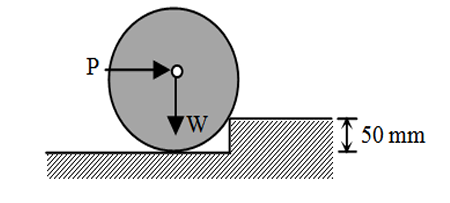
\includegraphics[width=0.5\linewidth]{GATE-CE-2018/28-1.png}
    \caption{}
    \label{28-1}
\end{figure}
All interfaces are assumed frictionless. The minimum value of $P$ is
\hfill{(GATE 2018)}
\begin{multicols}{4}
\begin{enumerate}
    \item 4.5 kN
    \item 5.0 kN
    \item 6.0 kN
    \item 7.5 kN
\end{enumerate}
\end{multicols}
\vspace{1cm}
\newpage
% Q.29
\item A plate in equilibrium is subjected to uniform stresses along its edges with magnitude $\sigma_{xx}=30$ MPa and $\sigma_{yy}=50$ MPa as shown in the figure.
\begin{figure}[h]
    \centering
    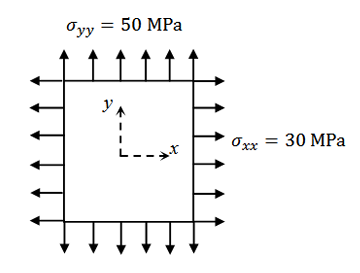
\includegraphics[width=0.5\linewidth]{GATE-CE-2018/29-1.png}
    \caption{}
    \label{29-1}
\end{figure}
The Young's modulus of the material is $2\times10^{11}$ N/m$^2$ and the Poisson's ratio is 0.3. If $\sigma_{zz}$ is negligibly small and assumed to be zero, then the strain $\varepsilon_{zz}$ is
\hfill{(GATE 2018)}
\begin{multicols}{4}
\begin{enumerate}
    \item -$120\times10^{-6}$
    \item -$60\times10^{-6}$
    \item $0.0$
    \item $120\times10^{-6}$
\end{enumerate}
\end{multicols}
\vspace{1cm}

% Q.30
\item The figure shows a simply supported beam $PQ$ of uniform flexural rigidity $EI$ carrying two moments $M$ and $2M$.
\begin{figure}[h]
    \centering
    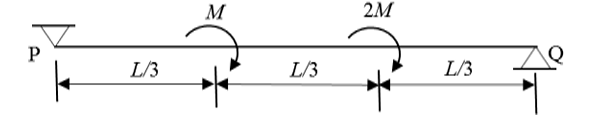
\includegraphics[width=0.5\linewidth]{GATE-CE-2018/30-1.png}
    \caption{}
    \label{30-1}
\end{figure}
The slope at $P$ will be
\hfill{(GATE 2018)}
\begin{multicols}{4}
\begin{enumerate}
    \item 0
    \item $ML/(9EI)$
    \item $ML/(6EI)$
    \item $ML/(3EI)$
\end{enumerate}
\end{multicols}
\vspace{1cm}
\newpage
% Q.31
\item A 0.5 m $\times$ 0.5 m square concrete pile is to be driven in a homogeneous clayey soil having undrained shear strength, $c_u = 50$ kPa and unit weight, $\gamma = 18.0$ kN/m$^3$. The design capacity of the pile is 500 kN. The adhesion factor $\alpha$ is given as 0.75. The length of the pile required for the above design load with a factor of safety of 2.0 is
\hfill{(GATE 2018)}
\begin{multicols}{4}
\begin{enumerate}
    \item 5.2 m
    \item 5.8 m
    \item 11.8 m
    \item 12.5 m
\end{enumerate}
\end{multicols}
\vspace{1cm}

% Q.32
\item A closed tank contains 0.5 m thick layer of mercury (specific gravity = 13.6) at the bottom. A 2.0 m thick layer of water lies above the mercury layer. A 3.0 m thick layer of oil (specific gravity = 0.6) lies above the water layer. The space above the oil layer contains air under pressure. The gauge pressure at the bottom of the tank is 196.2 kN/m$^2$. The density of water is 1000 kg/m$^3$ and the acceleration due to gravity is 9.81 m/s$^2$. The value of pressure in the air space is
\hfill{(GATE 2018)}
\begin{multicols}{4}
\begin{enumerate}
    \item 92.214 kN/m$^2$
    \item 95.644 kN/m$^2$
    \item 98.922 kN/m$^2$
    \item 99.321 kN/m$^2$
\end{enumerate}
\end{multicols}
\vspace{1cm}

% Q.33
\item A rapid sand filter comprising a number of filter beds is required to produce 99 MLD of potable water. Consider water loss during backwashing as 5\%, rate of filtration as 6.0 m/h and length to width ratio of filter bed as 1.35. The width of each filter bed is to be kept equal to 5.2 m. One additional filter bed is to be provided to take care of break-down, repair and maintenance. The total number of filter beds required will be
\hfill{(GATE 2018)}
\begin{multicols}{4}
\begin{enumerate}
    \item 19
    \item 20
    \item 21
    \item 22
\end{enumerate}
\end{multicols}
\vspace{1cm}

% Q.34
\item A priority intersection has a single-lane one-way traffic road crossing an undivided two-lane two-way traffic road. The traffic stream speed on the single-lane road is 20 kmph and the speed on the two-lane road is 50 kmph. The perception-reaction time is 2.5 s, coefficient of longitudinal friction is 0.38 and acceleration due to gravity is 9.81 m/s$^2$. A clear sight triangle has to be ensured at this intersection. The minimum lengths of the sides of the sight triangle along the two-lane road and the single-lane road, respectively will be
\hfill{(GATE 2018)}
\begin{multicols}{4}
\begin{enumerate}
    \item 50 m and 20 m
    \item 61 m and 18 m
    \item 111 m and 15 m
    \item 122 m and 36 m
\end{enumerate}
\end{multicols}
\vspace{1cm}

\newpage
% Q.35
\item The following details refer to a closed traverse:
\[
\begin{array}{|c|c|c|c|c|}
\hline
\text{Line} & \multicolumn{4}{c|}{\text{Consecutive coordinate}}\\
 & \text{Northing (m)} & \text{Southing (m)} & \text{Easting (m)} & \text{Westing (m)} \\
\hline
PQ & ---- & 437 & 173 & ---- \\
QR & 101 & ---- & 558 & ---- \\
RS & 419 & ---- & ---- & 96 \\
SP & ---- & 83 & ---- & 634 \\
\hline
\end{array}
\]
The length and direction (whole circle bearing) of closure, respectively are
\hfill{(GATE 2018)}
\begin{multicols}{4}
\begin{enumerate}
    \item 1 m and $90^\circ$
    \item 2 m and $90^\circ$
    \item 1 m and $270^\circ$
    \item 2 m and $270^\circ$
\end{enumerate}
\end{multicols}
\vspace{1cm}

% Q.36
\item A square area (on the surface of the earth) with side 100 m and uniform height, appears as 1 cm$^2$ on a vertical aerial photograph. The topographic map shows that a contour of 650 m passes through the area. If focal length of the camera lens is 150 mm, the height from which the aerial photograph was taken, is
\hfill{(GATE 2018)}
\begin{multicols}{4}
\begin{enumerate}
    \item 800 m
    \item 1500 m
    \item 2150 m
    \item 3150 m
\end{enumerate}
\end{multicols}
\vspace{1cm}

% Q.37
\item The solution at $x=1,~t=1$ of the partial differential equation $\dfrac{\partial^2 u}{\partial x^2}=25\dfrac{\partial^2 u}{\partial t^2}$ subject to initial conditions of $u(0)=3x$ and $\dfrac{\partial u}{\partial t}(0)=3$ is \underline{\hspace{3cm}}
\hfill{(GATE 2018)}
\vspace{1cm}

% Q.38
\item The solution (up to three decimal places) at $x=1$ of the differential equation $\dfrac{d^2 y}{dx^2}+2 \dfrac{dy}{dx}+y=0$ subject to boundary conditions $y(0)=1$ and $\dfrac{dy}{dx}(0) = -1$ is \underline{\hspace{3cm}}
\hfill{(GATE 2018)}
\vspace{1cm}

% Q.39
\item Variation of water depth ($y$) in a gradually varied open channel flow is given by the first order differential equation
\[
\dfrac{dy}{dx} = \dfrac{1-e^{-\frac{10}{3}\ln(y)}}{250-45e^{-3\ln(y)}}
\]
Given initial condition: $y(x=0) = 0.8$ m. The depth (in m, up to three decimal places) of flow at a downstream section at $x=1$ m from one calculation step of Single Step Euler Method is \underline{\hspace{3cm}}
\hfill{(GATE 2018)}
\vspace{1cm}

% Q.40
\item An RCC short column (with lateral ties) of rectangular cross section of 250 mm $\times$ 300 mm is furnished with four numbers of 16 mm diameter longitudinal bars. The grades of steel and concrete are Fe415 and M20, respectively. Neglect eccentricity effect. Considering limit state of collapse in compression (IS 456 : 2000), the axial load carrying capacity of the column (in kN, up to one decimal place) is \underline{\hspace{3cm}}
\hfill{(GATE 2018)}
\vspace{1cm}

% Q.41
\item An RCC beam of rectangular cross section has factored shear of 200 kN at its critical section. Its width $b$ is 250 mm and effective depth $d$ is 350 mm. Assume design shear strength $\tau_c$ of concrete as 0.62 N/mm$^2$ and maximum allowable shear stress $\tau_{c,max}$ in concrete as 2.8 N/mm$^2$. If two legged 10 mm diameter vertical stirrups of Fe250 grade steel are used, then the required spacing (in cm, up to one decimal place) as per limit state method will be \underline{\hspace{3cm}}
\hfill{(GATE 2018)}
\vspace{1cm}

% Q.42
\item The dimensions of a symmetrical welded I-section are shown in the figure.
\begin{figure}[h]
    \centering
    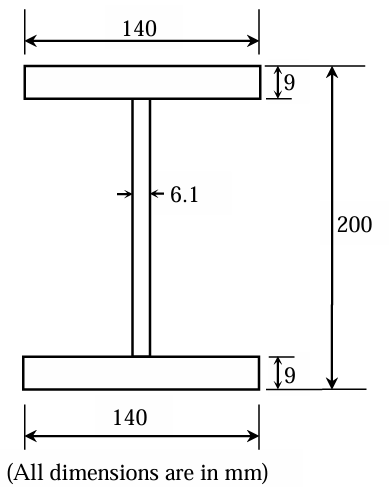
\includegraphics[width=0.5\linewidth]{GATE-CE-2018/42-1.png}
    \caption{}
    \label{42-1}
\end{figure}
The plastic section modulus about the weaker axis (in cm$^3$, up to one decimal place) is \underline{\hspace{3cm}}
\hfill{(GATE 2018)}
\vspace{1cm}
\newpage
% Q.43
\item Consider the deformable pin-jointed truss with loading, geometry and section properties as shown in the figure.
\begin{figure}[h]
    \centering
    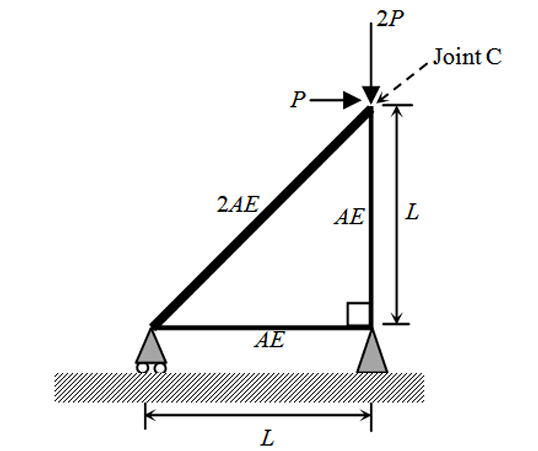
\includegraphics[width=0.5\linewidth]{GATE-CE-2018/43-1.png}
    \caption{}
    \label{43-1}
\end{figure}
Given that $E = 2 \times 10^{11}$ N/m$^2$, $A = 10$ mm$^2$, $L = 1$ m and $P = 1$ kN. The horizontal displacement of Joint C (in mm, up to one decimal place) is \underline{\hspace{3cm}}
\hfill{(GATE 2018)}
\vspace{1cm}

% Q.44
\item At a construction site, a contractor plans to make an excavation as shown in the figure.
\begin{figure}[h]
    \centering
    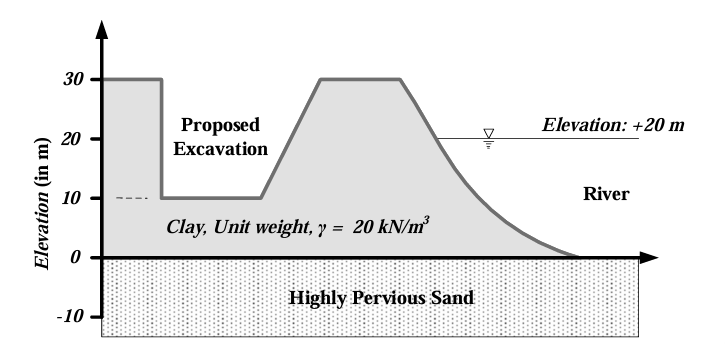
\includegraphics[width=0.5\linewidth]{GATE-CE-2018/44-1.png}
    \caption{}
    \label{44-1}
\end{figure}
The water level in the adjacent river is at an elevation of +20.0 m. Unit weight of water is 10 kN/m$^3$. The factor of safety (up to two decimal places) against sand boiling for the proposed excavation is \underline{\hspace{3cm}}
\hfill{(GATE 2018)}
\vspace{1cm}

% Q.45
\item A conventional drained triaxial compression test was conducted on a normally consolidated clay sample under an effective confining pressure of 200 kPa. The deviator stress at failure was found to be 400 kPa. An identical specimen of the same clay sample is isotropically consolidated to a confining pressure of 200 kPa and subjected to standard undrained triaxial compression test. If the deviator stress at failure is 150 kPa, the pore pressure developed (in kPa, up to one decimal place) is \underline{\hspace{3cm}}
\hfill{(GATE 2018)}
\vspace{1cm}

% Q.46
\item The void ratio of a soil is 0.55 at an effective normal stress of 140 kPa. The compression index of the soil is 0.25. In order to reduce the void ratio to 0.4, an increase in the magnitude of effective normal stress (in kPa, up to one decimal place) should be \underline{\hspace{3cm}}
\hfill{(GATE 2018)}
\vspace{1cm}

% Q.47
\item A rigid smooth retaining wall of height 7 m with vertical backface retains saturated clay as backfill. The saturated unit weight and undrained cohesion of the backfill are 17.2 kN/m$^3$ and 20 kPa, respectively. The difference in the active lateral forces on the wall (in kN per meter length of wall, up to two decimal places), before and after the occurrence of tension cracks is \underline{\hspace{3cm}}
\hfill{(GATE 2018)}
\vspace{1cm}

% Q.48
\item Rainfall depth over a watershed is monitored through six number of well distributed rain gauges. Gauged data are given below
\[
\begin{array}{|c|cccccc|}
\hline
\text{Rain Gauge Number} & 1 & 2 & 3 & 4 & 5 & 6 \\
\hline
\text{Rainfall Depth (mm)} & 470 & 465 & 435 & 525 & 480 & 510 \\
\text{Area of Thiessen Polygon ($\times 10^4$ m$^2$)} & 95 & 100 & 98 & 80 & 85 & 92 \\
\hline
\end{array}
\]
The Thiessen mean value (in mm, up to one decimal place) of the rainfall is \underline{\hspace{3cm}}
\hfill{(GATE 2018)}
\vspace{1cm}

% Q.49
\item The infiltration rate $f$ in a basin under ponding condition is given by $f = 30 + 10e^{-2t}$, where, $f$ is in mm/h and $t$ is time in hour. Total depth of infiltration (in mm, up to one decimal place) during the last 20 minutes of a storm of 30 minutes duration is \underline{\hspace{3cm}}
\hfill{(GATE 2018)}
\vspace{1cm}

% Q.50
\item In a laboratory, a flow experiment is performed over a hydraulic structure. The measured values of discharge and velocity are 0.05 m$^3$/s and 0.25 m/s, respectively. If the full scale structure (30 times bigger) is subjected to a discharge of 270 m$^3$/s, then the time scale (model to full scale) value (up to two decimal places) is \underline{\hspace{3cm}}
\hfill{(GATE 2018)}
\vspace{1cm}

% Q.51
\item A water sample analysis data is given below.
\[
\begin{array}{|c|c|c|}
\hline
\text{Ion} & \text{Concentration (mg/L)} & \text{Atomic Weight} \\
\hline
\text{Ca}^{2+} & 60 & 40 \\
\text{Mg}^{2+} & 30 & 24.31 \\
\text{HCO}_3^- & 400 & 61 \\
\hline
\end{array}
\]
The carbonate hardness (expressed as mg/L of CaCO$_3$, up to one decimal place) for the water sample is \underline{\hspace{3cm}}
\hfill{(GATE 2018)}
\vspace{1cm}
\newpage
% Q.52
\item The ultimate BOD ($L_0$) of a wastewater sample is estimated as 87\% of COD. The COD of this wastewater is 300 mg/L. Considering first order BOD reaction rate constant $k$ (use natural log) = 0.23 per day and temperature coefficient $\theta = 1.047$, the BOD value (in mg/L, up to one decimal place) after three days of incubation at 27$^\circ$C for this wastewater will be \underline{\hspace{3cm}}
\hfill{(GATE 2018)}
\vspace{1cm}

% Q.53
\item A waste activated sludge (WAS) is to be blended with green waste (GW). The carbon (C) and nitrogen (N) contents, per kg of WAS and GW, on dry basis are given in the table.\\
\[
\begin{array}{|c|c|c|}
\hline
\text{Parameter} & \text{WAS} & \text{GW} \\
\hline
\text{Carbon (g)} & 54 & 360 \\
\text{Nitrogen (g)} & 10 & 6 \\
\hline
\end{array}
\]
The ratio of WAS to GW required (up to two decimal places) to achieve a blended C:N ratio of 20:1 on dry basis is \underline{\hspace{3cm}}
\hfill{(GATE 2018)}
\vspace{1cm}

% Q.54
\item Given the following data: design life $n = 15$ years, lane distribution factor $D = 0.75$, annual rate of growth of commercial vehicles $r = 6\%$, vehicle damage factor $F = 4$ and initial traffic in the year of completion of construction $=3000$ Commercial Vehicles Per Day (CVPD). As per IRC:37-2012, the design traffic in terms of cumulative number of standard axles (in million standard axles, up to two decimal places) is \underline{\hspace{3cm}}
\hfill{(GATE 2018)}
\vspace{1cm}

% Q.55
\item An aircraft approaches the threshold of a runway strip at a speed of 200 km/h. The pilot decelerates the aircraft at a rate of 1.697 m/s$^2$ and takes 18 s to exit the runway strip. If the deceleration after exiting the runway is 1 m/s$^2$, then the distance (in m, up to one decimal place) of the gate position from the location of exit on the runway is \underline{\hspace{3cm}}
\hfill{(GATE 2018)}
\vspace{1cm}
\vspace{4cm}
\begin{center}
    \textbf{\Large END OF THE QUESTION PAPER}
\end{center}
\newpage
\begin{center}
    

\vspace{15cm}
\textbf{\LARGE SESSION 2}
\end{center}
\newpage

    
   




    
\end{enumerate}

\textbf{\large Q.1 - Q.5 carry one mark each}
\vspace{1cm}
\begin{enumerate}
    % Q.1
\item ``His face \underline{\hspace{1.5cm}} with joy when the solution of the puzzle was \underline{\hspace{1.5cm}} to him.''
\\The words that best fill the blanks in the above sentence are
\hfill{(GATE 2018)}
\begin{multicols}{4}
\begin{enumerate}
    \item shone, shown
    \item shone, shone
    \item shown, shone
    \item shown, shown
\end{enumerate}
\end{multicols}
\vspace{1cm}

% Q.2
\item ``Although it does contain some pioneering ideas, one would hardly characterize the work as \underline{\hspace{2cm}}.''
\\The word that best fills the blank in the above sentence is
\hfill{(GATE 2018)}
\begin{multicols}{4}
\begin{enumerate}
    \item innovative
    \item simple
    \item dull
    \item boring
\end{enumerate}
\end{multicols}
\vspace{1cm}

% Q.3
\item $a + \underbrace{a + a + \cdots + a}_{n \;\text{times}} = a^2b$ and $b + \underbrace{b + b + \cdots + b}_{m \;\text{times}} = ab^2$, where $a,b,n$ and $m$ are natural numbers. What is the value of\\
$\left(\underbrace{m + m + m + \cdots + m}_{n \;\text{times}}\right) \left(\underbrace{n + n + n + \cdots + n}_{m \;\text{times}}\right)$?
\hfill{(GATE 2018)}
\begin{multicols}{4}
\begin{enumerate}
    \item $2a^2b^2$
    \item $a^4b^4$
    \item $ab(a+b)$
    \item $a^2+b^2$
\end{enumerate}
\end{multicols}
\vspace{1cm}

% Q.4
\item A three-member committee has to be formed from a group of 9 people. How many such distinct committees can be formed?
\hfill{(GATE 2018)}
\begin{multicols}{4}
\begin{enumerate}
    \item 27
    \item 72
    \item 81
    \item 84
\end{enumerate}
\end{multicols}
\vspace{1cm}

% Q.5
\item For non-negative integers, $a, b, c$, what would be the value of $a+b+c$ if\\
$\log a + \log b + \log c = 0$?
\hfill{(GATE 2018)}
\begin{multicols}{4}
\begin{enumerate}
    \item 3
    \item 1
    \item 0
    \item $-1$
\end{enumerate}
\end{multicols}
\vspace{1cm}

\textbf{\large Q.6 - Q.10 carry two mark each}
\vspace{1cm}
% Q.6
\item In manufacturing industries, loss is usually taken to be proportional to the square of the deviation from a target. If the loss is Rs. 4900 for a deviation of 7 units, what would be the loss in Rupees for a deviation of 4 units from the target?
\hfill{(GATE 2018)}
\begin{multicols}{4}
\begin{enumerate}
    \item 400
    \item 1200
    \item 1600
    \item 2800
\end{enumerate}
\end{multicols}
\vspace{1cm}

% Q.7
\item A faulty wall clock is known to gain 15 minutes every 24 hours. It is synchronized to the correct time at 9 AM on 11$^{\text{th}}$ July. What will be the correct time to the nearest minute when the clock shows 2 PM on 15$^{\text{th}}$ July of the same year?
\hfill{(GATE 2018)}
\begin{multicols}{4}
\begin{enumerate}
    \item 12:45 PM
    \item 12:58 PM
    \item 1:00 PM
    \item 2:00 PM
\end{enumerate}
\end{multicols}
\vspace{1cm}

% Q.8
\item The annual average rainfall in a tropical city is 1000 mm. On a particular rainy day (24-hour period), the cumulative rainfall experienced by the city is shown in the graph. Over the 24-hour period, 50\% of the rainfall falling on a rooftop, which had an obstruction-free area of $50~\text{m}^2$, was harvested into a tank. What is the total volume of water collected in the tank in liters?
\begin{figure}[h]
    \centering
    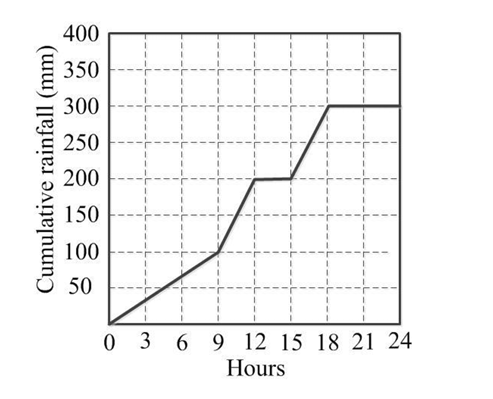
\includegraphics[width=0.5\linewidth]{GATE-CE-2018/8A-2.png}
    \caption{}
    \label{8a-2}
\end{figure}
\hfill{(GATE 2018)}
\begin{multicols}{4}
\begin{enumerate}
    \item 25,000
    \item 18,750
    \item 7,500
    \item 3,125
\end{enumerate}
\end{multicols}
\vspace{1cm}

% Q.9
\item Given that $\dfrac{\log P}{y-z} = \dfrac{\log Q}{z-x} = \dfrac{\log R}{x-y} = 10$ for $x \neq y \neq z$, what is the value of the product $PQR$?
\hfill{(GATE 2018)}
\begin{multicols}{4}
\begin{enumerate}
    \item 0
    \item 1
    \item $xyz$
    \item $10^{xyz}$
\end{enumerate}
\end{multicols}
\vspace{1cm}
\newpage
% Q.10
\item Each of the letters in the figure below represents a unique integer from 1 to 9. The letters are positioned in the figure such that each of $(A+B+C)$, $(C+D+E)$, $(E+F+G)$ and $(G+H+K)$ is equal to 13. Which integer does $E$ represent?
\begin{figure}
    \centering
    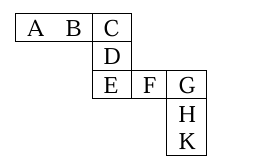
\includegraphics[width=0.5\linewidth]{GATE-CE-2018/10A-2.png}
    \caption{}
    \label{10a-2}
\end{figure}
\hfill{(GATE 2018)}
\begin{multicols}{4}
\begin{enumerate}
    \item 1
    \item 4
    \item 6
    \item 7
\end{enumerate}
\end{multicols}
\vspace{5cm}
\begin{center}
   \textbf{\large END OF THE QUESTION PAPER} 
\end{center}







    
\end{enumerate}
\newpage
\textbf{\large Q.1 - Q.25 carry one mark each}
\begin{enumerate}

\vspace{1cm}
% Q.1
\item The solution of the equation $x \dfrac{dy}{dx} + y = 0$ passing through the point $(1,1)$ is
\hfill{(GATE 2018)}

\begin{enumerate}
    \item $x$
    \item $x^2$
    \item $x^{-1}$
    \item $x^{-2}$
\end{enumerate}

\vspace{1cm}

% Q.2
\item The graph of a function $f(x)$ is shown in the figure.
\begin{figure}[h]
    \centering
    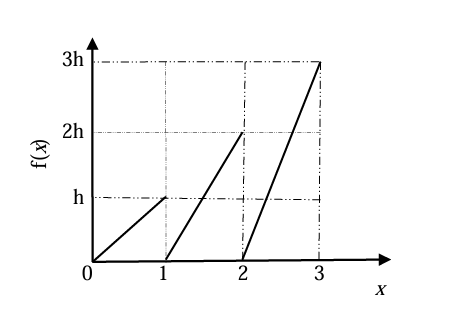
\includegraphics[width=0.5\linewidth]{GATE-CE-2018/2-2.png}
    \caption{}
    \label{2-2}
\end{figure}
For $f(x)$ to be a valid probability density function, the value of $h$ is
\hfill{(GATE 2018)}
\begin{multicols}{4}
\begin{enumerate}
    \item 1/3
    \item 2/3
    \item 1
    \item 3
\end{enumerate}
\end{multicols}
\vspace{1cm}

% Q.3
\item A probability distribution with right skew is shown in the figure.
\begin{figure}
    \centering
    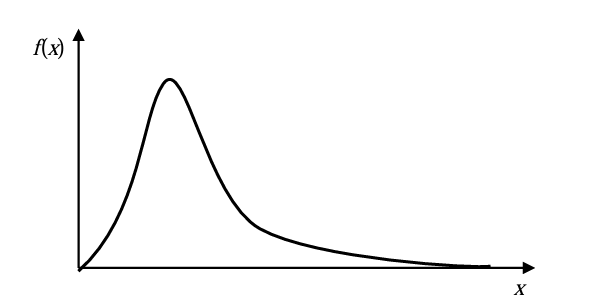
\includegraphics[width=0.5\linewidth]{GATE-CE-2018/3-2.png}
    \caption{}
    \label{3-2}
\end{figure}
The correct statement for the probability distribution is
\hfill{(GATE 2018)}

\begin{enumerate}
    \item Mean is equal to mode
    \item Mean is greater than median but less than mode
    \item Mean is greater than median and mode
    \item Mode is greater than median
\end{enumerate}

\vspace{1cm}

% Q.4
\item All the members of the planar truss (see figure), have the same properties in terms of area of cross-section ($A$) and modulus of elasticity ($E$).
\begin{figure}[h]
    \centering
    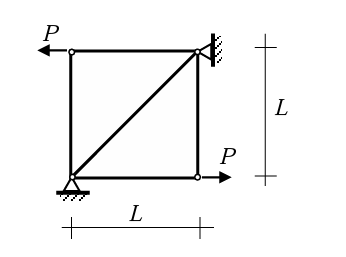
\includegraphics[width=0.5\linewidth]{GATE-CE-2018/4-2.png}
    \caption{}
    \label{4-2}
\end{figure}
For the loads shown on the truss, the statement that correctly represents the nature of forces in the members of the truss is:
\hfill{(GATE 2018)}

\begin{enumerate}
    \item There are 3 members in tension, and 2 members in compression
    \item There are 2 members in tension, 2 members in compression, and 1 zero-force member
    \item There are 2 members in tension, 1 member in compression, and 2 zero-force members
    \item There are 2 members in tension, and 3 zero-force members
\end{enumerate}

\vspace{1cm}

% Q.5
\item The setting time of cement is determined using
\hfill{(GATE 2018)}

\begin{enumerate}
    \item Le Chatelier apparatus
    \item Briquette testing apparatus
    \item Vicat apparatus
    \item Casagrande's apparatus
\end{enumerate}

\vspace{1cm}

% Q.6
\item A structural member subjected to compression, has both translation and rotation restrained at one end, while only translation is restrained at the other end. As per IS 456:2000, the effective length factor recommended for design is
\hfill{(GATE 2018)}
\begin{multicols}{4}
\begin{enumerate}
    \item 0.50
    \item 0.65
    \item 0.70
    \item 0.80
\end{enumerate}
\end{multicols}
\vspace{1cm}
\newpage
% Q.7
\item A vertical load of 10 kN acts on a hinge located at a distance of $L/4$ from the roller support Q of a beam of length $L$ (see figure).
\begin{figure}[h]
    \centering
    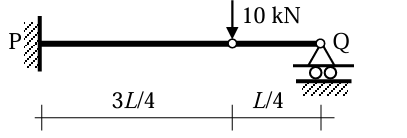
\includegraphics[width=0.5\linewidth]{GATE-CE-2018/7-2.png}
    \caption{}
    \label{7-2}
\end{figure}
The vertical reaction at support Q is
\hfill{(GATE 2018)}
\begin{multicols}{4}
\begin{enumerate}
    \item 0.0 kN
    \item 2.5 kN
    \item 7.5 kN
    \item 10.0 kN
\end{enumerate}
\end{multicols}
\vspace{1cm}

% Q.8
\item A flownet below a dam consists of 24 equipotential drops and 7 flow channels. The difference between the upstream and downstream water levels is $6$ m. The length of the flow line adjacent to the toe of the dam at exit is $1$ m. The specific gravity and void ratio of the soil below the dam are $2.70$ and $0.70$, respectively. The factor of safety against piping is
\hfill{(GATE 2018)}
\begin{multicols}{4}
\begin{enumerate}
    \item 1.67
    \item 2.55
    \item 3.4
    \item 4
\end{enumerate}
\end{multicols}
\vspace{1cm}

% Q.9
\item The contact pressure and settlement distribution for a footing are shown in the figure.
\begin{figure}[h]
    \centering
    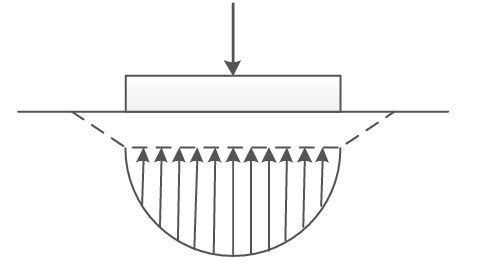
\includegraphics[width=0.5\linewidth]{GATE-CE-2018/9-2.png}
    \caption{}
    \label{9-2}
\end{figure}
The figure corresponds to a
\hfill{(GATE 2018)}
\begin{multicols}{4}
\begin{enumerate}
    \item rigid footing on granular soil
    \item flexible footing on granular soil
    \item flexible footing on saturated clay
    \item rigid footing on cohesive soil
\end{enumerate}
\end{multicols}
\vspace{1cm}
\newpage
% Q.10
\item Which one of the following statements is \textbf{NOT} correct?
\hfill{(GATE 2018)}
\begin{enumerate}
    \item When the water content of soil lies between its liquid limit and plastic limit, the soil is said to be in plastic state.
    \item Boussinesq's theory is used for the analysis of stratified soil.
    \item The inclination of stable slope in cohesive soil can be greater than its angle of internal friction.
    \item For saturated dense fine sand, after applying overburden correction, if the Standard Penetration Test value exceeds 15, dilatancy correction is to be applied.
\end{enumerate}
\vspace{1cm}

% Q.11
\item The clay mineral, whose structural units are held together by potassium bond is
\hfill{(GATE 2018)}
\begin{multicols}{4}
\begin{enumerate}
    \item Halloysite
    \item Illite
    \item Kaolinite
    \item Smectite
\end{enumerate}
\end{multicols}
\vspace{1cm}

% Q.12
\item Dupuit's assumptions are valid for
\hfill{(GATE 2018)}
\begin{multicols}{4}
\begin{enumerate}
    \item artesian aquifer
    \item confined aquifer
    \item leaky aquifer
    \item unconfined aquifer
\end{enumerate}
\end{multicols}
\vspace{1cm}

% Q.13
\item For a given discharge in an open channel, there are two depths which have the same specific energy. These two depths are known as
\hfill{(GATE 2018)}
\begin{multicols}{4}
\begin{enumerate}
    \item alternate depths
    \item critical depths
    \item normal depths
    \item sequent depths
\end{enumerate}
\end{multicols}
\vspace{1cm}

% Q.14
\item As per IS 10500:2012, for drinking water in the absence of alternate source of water, the permissible limits for chloride and sulphate, in mg/L, respectively are
\hfill{(GATE 2018)}
\begin{multicols}{4}
\begin{enumerate}
    \item 250 and 200
    \item 1000 and 400
    \item 200 and 250
    \item 500 and 1000
\end{enumerate}
\end{multicols}
\vspace{1cm}
\newpage
% Q.15
\item In the figures, Group I represents the atmospheric temperature profiles (P, Q, R and S) and Group II represents dispersion of pollutants from a smoke stack (1, 2, 3 and 4). In the figures of Group I, the dashed line represents the dry adiabatic lapse rate, whereas the horizontal axis represents temperature and the vertical axis represents the altitude.
\begin{figure}[h]
    \centering
    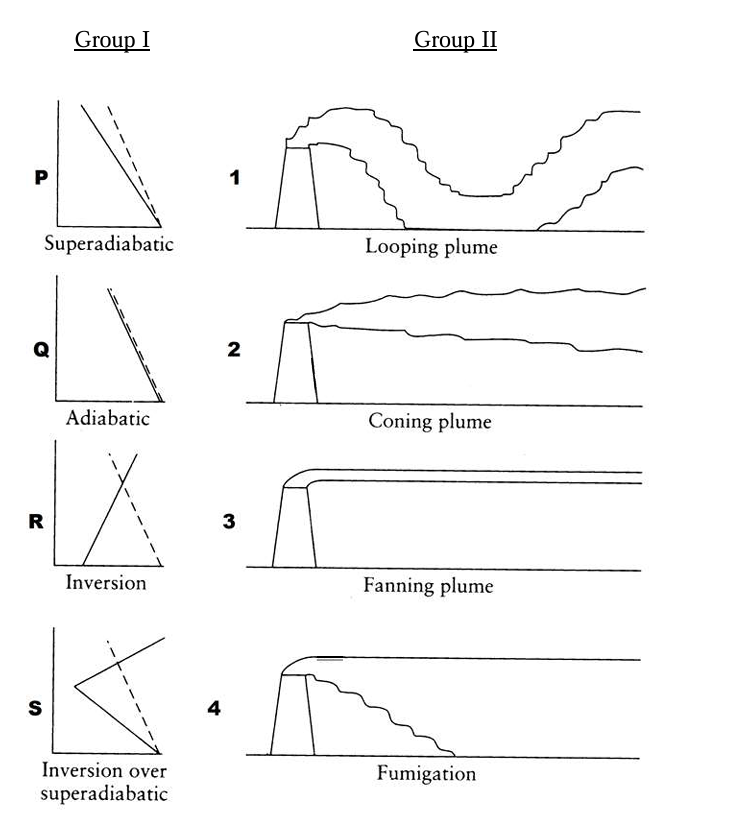
\includegraphics[width=0.5\linewidth]{GATE-CE-2018/15-2.png}
    \caption{}
    \label{15-2}
\end{figure}
The correct match is
\hfill{(GATE 2018)}
\begin{multicols}{4}
\begin{enumerate}
    \item P-1, Q-2, R-3, S-4
    \item P-1, Q-2, R-4, S-3
    \item P-1, Q-4, R-3, S-2
    \item P-3, Q-1, R-2, S-4
\end{enumerate}
\end{multicols}
\vspace{1cm}
\newpage
% Q.16
\item Peak Hour Factor (PHF) is used to represent the proportion of peak sub-hourly traffic flow within the peak hour. If 15-minute sub-hours are considered, the theoretically possible range of PHF will be
\hfill{(GATE 2018)}
\begin{multicols}{4}
\begin{enumerate}
    \item 0 to 1.0
    \item 0.25 to 0.75
    \item 0.25 to 1.0
    \item 0.5 to 1.0
\end{enumerate}
\end{multicols}
\vspace{1cm}

% Q.17
\item As per IRC:37-2012, in order to control subgrade rutting in flexible pavements, the parameter to be considered is
\hfill{(GATE 2018)}
\begin{multicols}{4}
\begin{enumerate}
    \item horizontal tensile strain at the bottom of bituminous layer
    \item vertical compressive strain on top of subgrade
    \item vertical compressive stress on top of granular layer
    \item vertical deflection at the surface of the pavement
\end{enumerate}
\end{multicols}
\vspace{1cm}

% Q.18
\item The initial concavity in the load-penetration curve of a CBR test is \textbf{NOT} due to
\hfill{(GATE 2018)}

\begin{enumerate}
    \item uneven top surface
    \item high impact at start of loading
    \item inclined penetration plunger
    \item soft top layer of soaked soil
\end{enumerate}

\vspace{1cm}

% Q.19
\item Probability (up to one decimal place) of consecutively picking $3$ red balls without replacement from a box containing $5$ red balls and $1$ white ball is \underline{\hspace{3cm}}
\hfill{(GATE 2018)}
\vspace{1cm}

% Q.20
\item The quadratic equation $2x^2 - 3x + 3 = 0$ is to be solved numerically starting with an initial guess as $x_0=2$. The new estimate of $x$ after the first iteration using Newton-Raphson method is \underline{\hspace{3cm}}
\hfill{(GATE 2018)}
\vspace{1cm}

% Q.21
\item As per IS 456:2000, the minimum percentage of tension reinforcement (up to two decimal places) required in reinforced-concrete beams of rectangular cross-section (considering effective depth in the calculation of area) using Fe500 grade steel is \underline{\hspace{3cm}}
\hfill{(GATE 2018)}
\vspace{1cm}

% Q.22
\item A reinforced-concrete slab with effective depth of $80$ mm is simply supported at two opposite ends on $230$ mm thick masonry walls. The centre-to-centre distance between the walls is $3.3$ m. As per IS 456 : 2000, the effective span of the slab (in m, up to two decimal places) is \underline{\hspace{3cm}}
\hfill{(GATE 2018)}
\vspace{1cm}

% Q.23
\item A fillet weld is simultaneously subjected to factored normal and shear stresses of $120$ MPa and $50$ MPa, respectively. As per IS 800:2007, the equivalent stress (in MPa, up to two decimal places) is \underline{\hspace{3cm}}
\hfill{(GATE 2018)}
\vspace{1cm}
\newpage
% Q.24
\item The intensity of irrigation for the \textit{Kharif} season is 50\% for an irrigation project with culturable command area of 50,000 hectares. The duty for the \textit{Kharif} season is 1000 hectare/cumec. Assuming transmission loss of 10\%, the required discharge (in cumec, up to two decimal places) at the head of the canal is \underline{\hspace{3cm}}
\hfill{(GATE 2018)}
\vspace{1cm}

% Q.25
\item A culvert is designed for a flood frequency of 100 years and a useful life of 20 years. The risk involved in the design of the culvert (in percentage, up to two decimal places) is \underline{\hspace{3cm}}
\hfill{(GATE 2018)}
\vspace{1cm}

% Q.26
\item The matrix $
\myvec{
2 & -4 \\
4 & -2
}
$ has
\hfill{(GATE 2018)}
\begin{multicols}{2}
\begin{enumerate}
    \item real eigenvalues and eigenvectors
    \item real eigenvalues but complex eigenvectors
    \item complex eigenvalues but real eigenvectors
    \item complex eigenvalues and eigenvectors
\end{enumerate}
\end{multicols}
\vspace{1cm}

% Q.27
\item The Laplace transform $F(s)$ of the exponential function, $f(t) = e^{at}$ when $t \ge 0$, where $a$ is a constant and $(s-a)>0$, is
\hfill{(GATE 2018)}
\begin{multicols}{2}
\begin{enumerate}
    \item $\dfrac{1}{s+a}$
    \item $\dfrac{1}{s-a}$
    \item $\dfrac{1}{a-s}$
    \item $\infty$
\end{enumerate}
\end{multicols}
\vspace{1cm}

% Q.28
\item The rank of the following matrix is
\[
\myvec{
1 & 1 & 0 & -2 \\
2 & 0 & 2 & 2 \\
4 & 1 & 3 & 1 \\
}
\]
\hfill{(GATE 2018)}
\begin{multicols}{4}
\begin{enumerate}
    \item 1
    \item 2
    \item 3
    \item 4
\end{enumerate}
\end{multicols}
\vspace{1cm}
\newpage
% Q.29
\item Two rigid bodies of mass 5 kg and 4 kg are at rest on a frictionless surface until acted upon by a force of 36 N as shown in the figure. The contact force generated between the two bodies is
\begin{figure}[h]
    \centering
    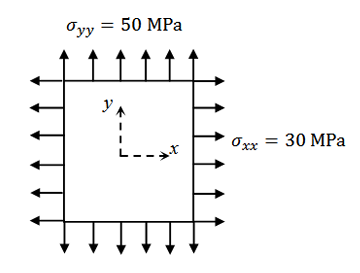
\includegraphics[width=0.5\linewidth]{GATE-CE-2018/29-1.png}
    \caption{}
    \label{29-2}
\end{figure}
\hfill{(GATE 2018)}
\begin{multicols}{4}
\begin{enumerate}
    \item 4.0 N
    \item 7.2 N
    \item 9.0 N
    \item 16.0 N
\end{enumerate}
\end{multicols}
\vspace{1cm}

\newpage
% Q.30
\item Four bolts P, Q, R and S of equal diameter are used for a bracket subjected to a load of 130 kN as shown in the figure.
\begin{figure}[h]
    \centering
    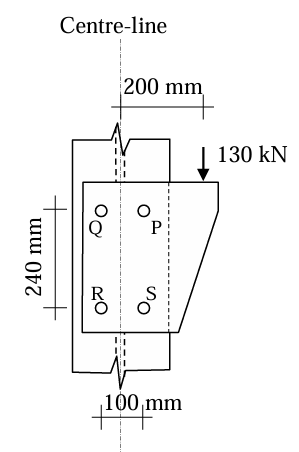
\includegraphics[width=0.5\linewidth]{GATE-CE-2018/30-2.png}
    \caption{}
    \label{30-2}
\end{figure}
The force in bolt P is
\hfill{(GATE 2018)}
\begin{multicols}{4}
\begin{enumerate}
    \item 32.50 kN
    \item 69.32 kN
    \item 82.50 kN
    \item 119.32 kN
\end{enumerate}
\end{multicols}
\vspace{1cm}

% Q.31
\item A singly-reinforced rectangular concrete beam of width 300 mm and effective depth 400 mm is to be designed using M25 grade concrete and Fe500 grade reinforcing steel. For the beam to be under-reinforced, the maximum number of 16 mm diameter reinforcing bars that can be provided is
\hfill{(GATE 2018)}
\begin{multicols}{4}
\begin{enumerate}
    \item 3
    \item 4
    \item 5
    \item 6
\end{enumerate}
\end{multicols}
\vspace{1cm}
\newpage
% Q.32
\item A 3 m high vertical earth retaining wall retains a dry granular backfill with angle of internal friction of $30^\circ$ and unit weight of $20$ kN/m$^3$. If the wall is prevented from yielding (no movement), the total horizontal thrust (in kN per unit length) on the wall is
\hfill{(GATE 2018)}
\begin{multicols}{4}
\begin{enumerate}
    \item 0
    \item 30
    \item 45
    \item 270
\end{enumerate}
\end{multicols}
\vspace{1cm}

% Q.33
\item Three soil specimens (Soil 1, Soil 2 and Soil 3), each 150 mm long and 100 mm diameter, are placed in series in a constant head flow set-up as shown in the figure. Suitable screens are provided at the boundaries of the specimens to keep them intact. The values of coefficient of permeability of Soil 1, Soil 2 and Soil 3 are 0.01, 0.003 and 0.03 cm/s, respectively.
\begin{figure}[h]
    \centering
    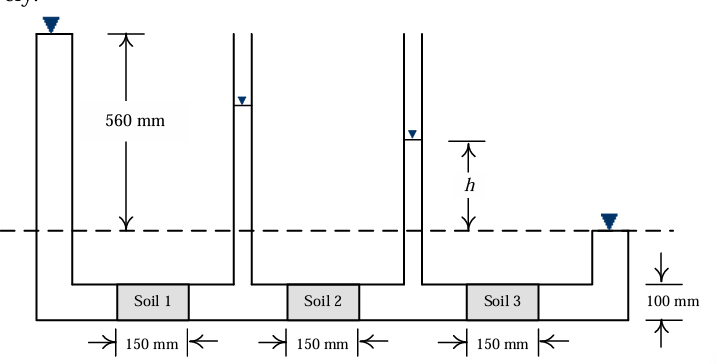
\includegraphics[width=0.5\linewidth]{GATE-CE-2018/33-2.png}
    \caption{}
    \label{33-2}
\end{figure}
The value of $h$ in the set-up is
\hfill{(GATE 2018)}
\begin{multicols}{4}
\begin{enumerate}
    \item 0 mm
    \item 40 mm
    \item 255 mm
    \item 560 mm
\end{enumerate}
\end{multicols}
\vspace{1cm}

% Q.34
\item In a 5 m wide rectangular channel, the velocity $u$ distribution in the vertical direction $y$ is given by $u=1.25y^{0.6}$. The distance $y$ is measured from the channel bed. If the flow depth is $2~$m, the discharge per unit width of the channel is
\hfill{(GATE 2018)}
\begin{multicols}{4}
\begin{enumerate}
    \item 2.40 m$^3$/s/m
    \item 2.80 m$^3$/s/m
    \item 3.27 m$^3$/s/m
    \item 12.02 m$^3$/s/m
\end{enumerate}
\end{multicols}
\vspace{1cm}

% Q.35
\item A car follows a slow moving truck (travelling at a speed of 10 m/s) on a two-lane two-way highway. The car reduces its speed to 10 m/s and follows the truck maintaining a distance of 16 m from the truck. On finding a clear gap in the opposing traffic stream, the car accelerates at an average rate of 4 m/s$^2$, overtakes the truck and returns to its original lane. When it returns to its original lane, the distance between the car and the truck is 16 m. The total distance covered by the car during this period (from the time it leaves its lane and subsequently returns to its lane after overtaking) is
\hfill{(GATE 2018)}
\begin{multicols}{4}
\begin{enumerate}
    \item 64 m
    \item 72 m
    \item 128 m
    \item 144 m
\end{enumerate}
\end{multicols}
\vspace{1cm}

% Q.36
\item A level instrument at a height of 1.320~m has been placed at a station having a Reduced Level (RL) of 112.565~m. The instrument reads $-2.835$~m on a levelling staff held at the bottom of a bridge deck. The RL (in m) of the bottom of the bridge deck is
\hfill{(GATE 2018)}
\begin{multicols}{4}
\begin{enumerate}
    \item 116.720
    \item 116.080
    \item 114.080
    \item 111.050
\end{enumerate}
\end{multicols}
\vspace{1cm}

% Q.37
\item The value (up to two decimal places) of a line integral $\int_C \vec{F}(\vec{r})\cdot d\vec{r}$, for $\vec{F}(\vec{r}) = x^2\vec{i} + y^2\vec{j}$ along $C$ which is a straight line joining (0,0) to (1,1) is \underline{\hspace{3cm}}
\hfill{(GATE 2018)}
\vspace{1cm}

% Q.38
\item An 8 m long simply-supported elastic beam of rectangular cross-section (100 mm $\times$ 200 mm) is subjected to a uniformly distributed load of 10 kN/m over its entire span. The maximum principal stress (in MPa, up to two decimal places) at a point located at the extreme compression edge of a cross-section and at 2 m from the support is \underline{\hspace{3cm}}
\hfill{(GATE 2018)}
\vspace{1cm}

% Q.39
\item A prismatic beam P-Q-R of flexural rigidity $EI = 1 \times 10^4$ kNm$^2$ is subjected to a moment of $180$ kNm at Q as shown in the figure.
\begin{figure}[h]
    \centering
    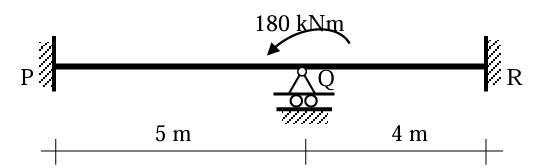
\includegraphics[width=0.5\linewidth]{GATE-CE-2018/39-2.png}
    \caption{}
    \label{39-2}
\end{figure}
The rotation at Q (in rad, up to two decimal places) is \underline{\hspace{3cm}}
\hfill{(GATE 2018)}
\vspace{1cm}

% Q.40
\item A prismatic propped cantilever beam of span $L$ and plastic moment capacity $M_p$ is subjected to a concentrated load at its mid-span. If the collapse load of the beam is $\alpha \dfrac{M_p}{L}$, the value of $\alpha$ is \underline{\hspace{3cm}}
\hfill{(GATE 2018)}
\vspace{1cm}

% Q.41
\item A $6$ m long simply-supported beam is prestressed as shown in the figure.
\begin{figure}[h]
    \centering
    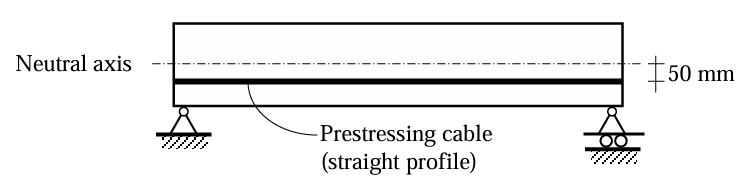
\includegraphics[width=0.5\linewidth]{GATE-CE-2018/41-2.png}
    \caption{}
    \label{41-2}
\end{figure}
The beam carries a uniformly distributed load of $6$ kN/m over its entire span. If the effective flexural rigidity $EI=2\times10^4$ kNm$^2$ and the effective prestressing force is 200 kN, the net increase in length of the prestressing cable (in mm, up to two decimal places) is \underline{\hspace{3cm}}
\hfill{(GATE 2018)}
\vspace{1cm}

% Q.42
\item A cable PQ of length $25$ m is supported at two ends at the same level as shown in the figure. The horizontal distance between the supports is $20$ m. A point load of $150$ kN is applied at point $R$ which divides it into two equal parts.
\begin{figure}[h]
    \centering
    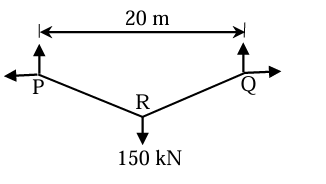
\includegraphics[width=0.5\linewidth]{GATE-CE-2018/42-2.png}
    \caption{}
    \label{42-2}
\end{figure}
Neglecting the self-weight of the cable, the tension (in kN, integer value) in the cable due to the applied load will be \underline{\hspace{3cm}}
\hfill{(GATE 2018)}
\vspace{1cm}

% Q.43
\item The compression curve (void ratio, $e$ vs. effective stress, $\sigma_v'$) for a certain clayey soil is a straight line in a semi-logarithmic plot and it passes through the points $(e=1.2; \sigma_v'=50$ kPa) and $(e=0.6; \sigma_v'=800$ kPa$)$. The compression index (up to two decimal places) of the soil is \underline{\hspace{3cm}}
\hfill{(GATE 2018)}
\vspace{1cm}

% Q.44
\item The total horizontal and vertical stresses at a point X in a saturated sandy medium are 170 kPa and 300 kPa, respectively. The static pore-water pressure is 30 kPa. At failure, the excess pore-water pressure is measured to be 94.50 kPa, and the shear stresses on the vertical and horizontal planes passing through the point X are zero. Effective cohesion is 0 kPa and effective angle of internal friction is $36^\circ$. The shear strength (in kPa, up to two decimal places) at point X is \underline{\hspace{3cm}}
\hfill{(GATE 2018)}
\vspace{1cm}
\newpage
% Q.45
\item A group of nine piles in a $3\times 3$ square pattern is embedded in a soil strata comprising dense sand and underlying recently filled clay layer, as shown in the figure. The perimeter of an individual pile is 126 cm. The size of pile group is $240$ cm $\times$ $240$ cm. The recently filled clay has undrained shear strength of 15 kPa and unit weight of 16 kN/m$^3$.
\begin{figure}[h]
    \centering
    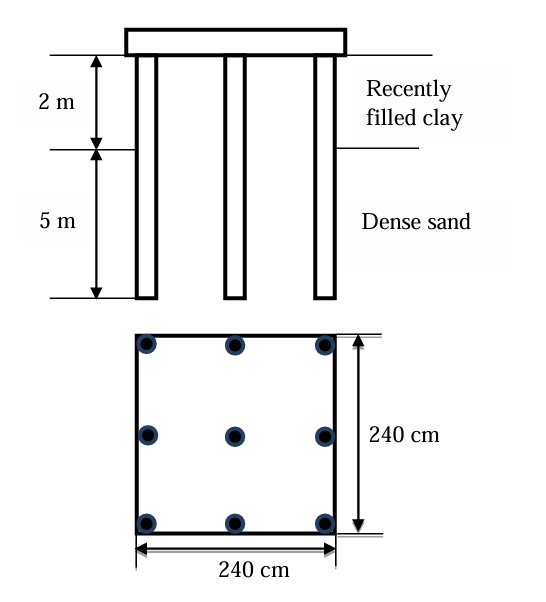
\includegraphics[width=0.5\linewidth]{GATE-CE-2018/45-2.png}
    \caption{}
    \label{45-2}
\end{figure}
The negative frictional load (in kN, up to two decimal places) acting on the pile group is \underline{\hspace{3cm}}
\hfill{(GATE 2018)}
\vspace{1cm}

% Q.46
\item A three-fluid system (immiscible) is connected to a vacuum pump. The specific gravity values of the fluids (S$_1$, S$_2$) are given in the figure.
\begin{figure}[h]
    \centering
    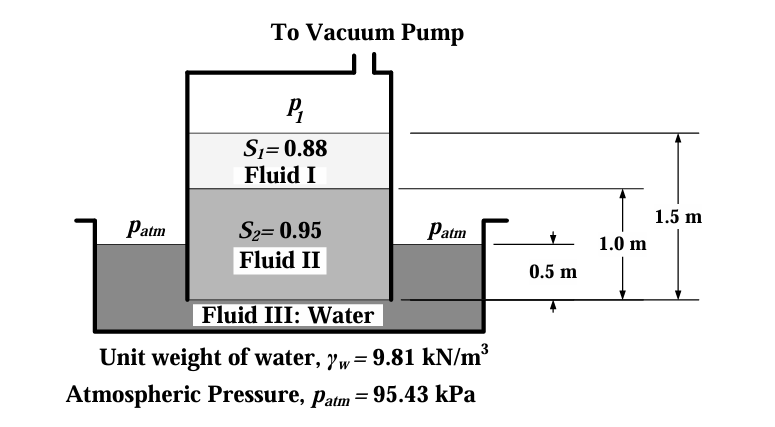
\includegraphics[width=0.5\linewidth]{GATE-CE-2018/46-2.png}
    \caption{Caption}
    \label{46-2}
\end{figure}[]
The gauge pressure value (in kN/m$^2$, up to two decimal places) of $p_1$ is \underline{\hspace{3cm}}
\hfill{(GATE 2018)}
\vspace{1cm}

% Q.47
\item The total rainfall in a catchment of area 1000 km$^2$, during a 6 h storm, is 19 cm. The surface runoff due to this storm computed from triangular direct runoff hydrograph is $1\times 10^8$ m$^3$. The $\phi_{index}$ for this storm (in cm/h, up to one decimal place) is \underline{\hspace{3cm}}
\hfill{(GATE 2018)}
\vspace{1cm}

% Q.48
\item A rough pipe of 0.5 m diameter, 300 m length and roughness height of 0.25 mm, carries water (kinematic viscosity $=0.9\times 10^{-6}$ m$^2$/s) with velocity of 3 m/s. Friction factor ($f$) for laminar flow is given by $f=64/Re$, and for turbulent flow it is given by $\dfrac{1}{\sqrt{f}}=2\log_{10}\left(\dfrac{r}{k}\right)+1.74$, where $Re$ = Reynolds number, $r$ = radius of pipe, $k$ = roughness height and $g=9.81$ m/s$^2$. The head loss (in m, up to three decimal places) in the pipe due to friction is \underline{\hspace{3cm}}
\hfill{(GATE 2018)}
\vspace{1cm}

% Q.49
\item A flocculation tank contains 1800 m$^3$ of water, which is mixed using paddles at an average velocity gradient $G$ of $100$/s. The water temperature and the corresponding dynamic viscosity are $30^\circ$C and $0.798\times 10^{-3}$ Ns/m$^2$, respectively. The theoretical power required to achieve the stated value of $G$ (in kW, up to two decimal places) is \underline{\hspace{3cm}}
\hfill{(GATE 2018)}
\vspace{1cm}

% Q.50
\item A coal containing 2\% sulfur is burned completely to ash in a brick kiln at a rate of 30 kg/min. The sulfur content in the ash was found to be 6\% of the initial amount of sulfur present in the coal fed to the brick kiln. The molecular weights of S, H and O are 32, 1 and 16 g/mole, respectively. The annual rate of sulfur dioxide (SO$_2$) emission from the kiln (in tonnes/year, up to two decimal places) is \underline{\hspace{3cm}}
\hfill{(GATE 2018)}
\vspace{1cm}

% Q.51
\item At a small water treatment plant which has 4 filters, the rates of filtration and backwashing are 200 m$^3$/d/m$^2$ and 1000 m$^3$/d/m$^2$, respectively. Backwashing is done for 15 min per day. The maturation, which occurs initially as the filter is put back into service after cleaning, takes 30 min. It is proposed to recover the water being wasted during backwashing and maturation. The percentage increase in the filtered water produced (up to two decimal places) would be \underline{\hspace{3cm}}
\hfill{(GATE 2018)}
\vspace{1cm}

% Q.52
\item A schematic flow diagram of a completely mixed biological reactor with provision for recycling of solids is shown in the figure.
\begin{figure}[h]
    \centering
    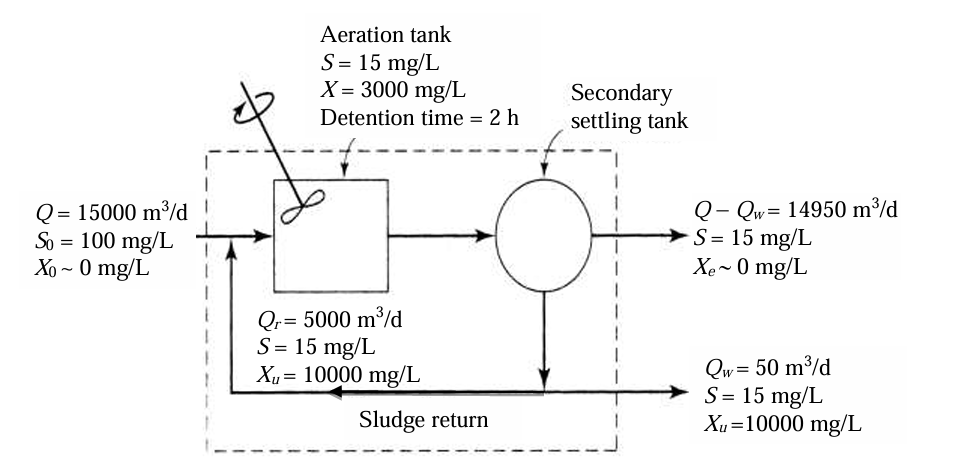
\includegraphics[width=0.5\linewidth]{GATE-CE-2018/52-2.png}
    \caption{}
    \label{52-2}
\end{figure}
The mean cell residence time (in days, up to one decimal place) is \underline{\hspace{3cm}}
\hfill{(GATE 2018)}
\vspace{1cm}

% Q.53
\item The space mean speed (kmph) and density (vehicles/km) of a traffic stream are linearly related. The free flow speed and jam density are 80 kmph and 100 vehicles/km respectively. The traffic flow (in vehicles/h, up to one decimal place) corresponding to a speed of 40 kmph is \underline{\hspace{3cm}}
\hfill{(GATE 2018)}
\vspace{1cm}

% Q.54
\item A 7.5 m wide two-lane road on a plain terrain is to be laid along a horizontal curve of radius 510 m. For a design speed of 100 kmph, super-elevation is provided as per IRC:73-1980. Consider acceleration due to gravity as 9.81 m/s$^2$. The level difference between the inner and outer edges of the road (in m, up to three decimal places) is \underline{\hspace{3cm}}
\hfill{(GATE 2018)}
\vspace{1cm}

% Q.55
\item An aerial photograph of a terrain having an average elevation of 1400 m is taken at a scale of 1:7500. The focal length of the camera is 15 cm. The altitude of the flight above mean sea level (in m, up to one decimal place) is \underline{\hspace{3cm}}
\hfill{(GATE 2018)}
\vspace{1cm}












   
\end{enumerate}






\end{document}